\documentclass{scrartcl}

\usepackage{graphicx}
\title{ Ich als Musiker }
\author{ Quang Thanh Ta }
\date{\today}

\usepackage[german]{babel}
\usepackage[backend=biber,style=alphabetic,natbib=true,hyperref=true]{biblatex}
\addbibresource{literatur-ta.bib}

%%% Begin document
\begin{document}
\maketitle

\begin{figure}[h]
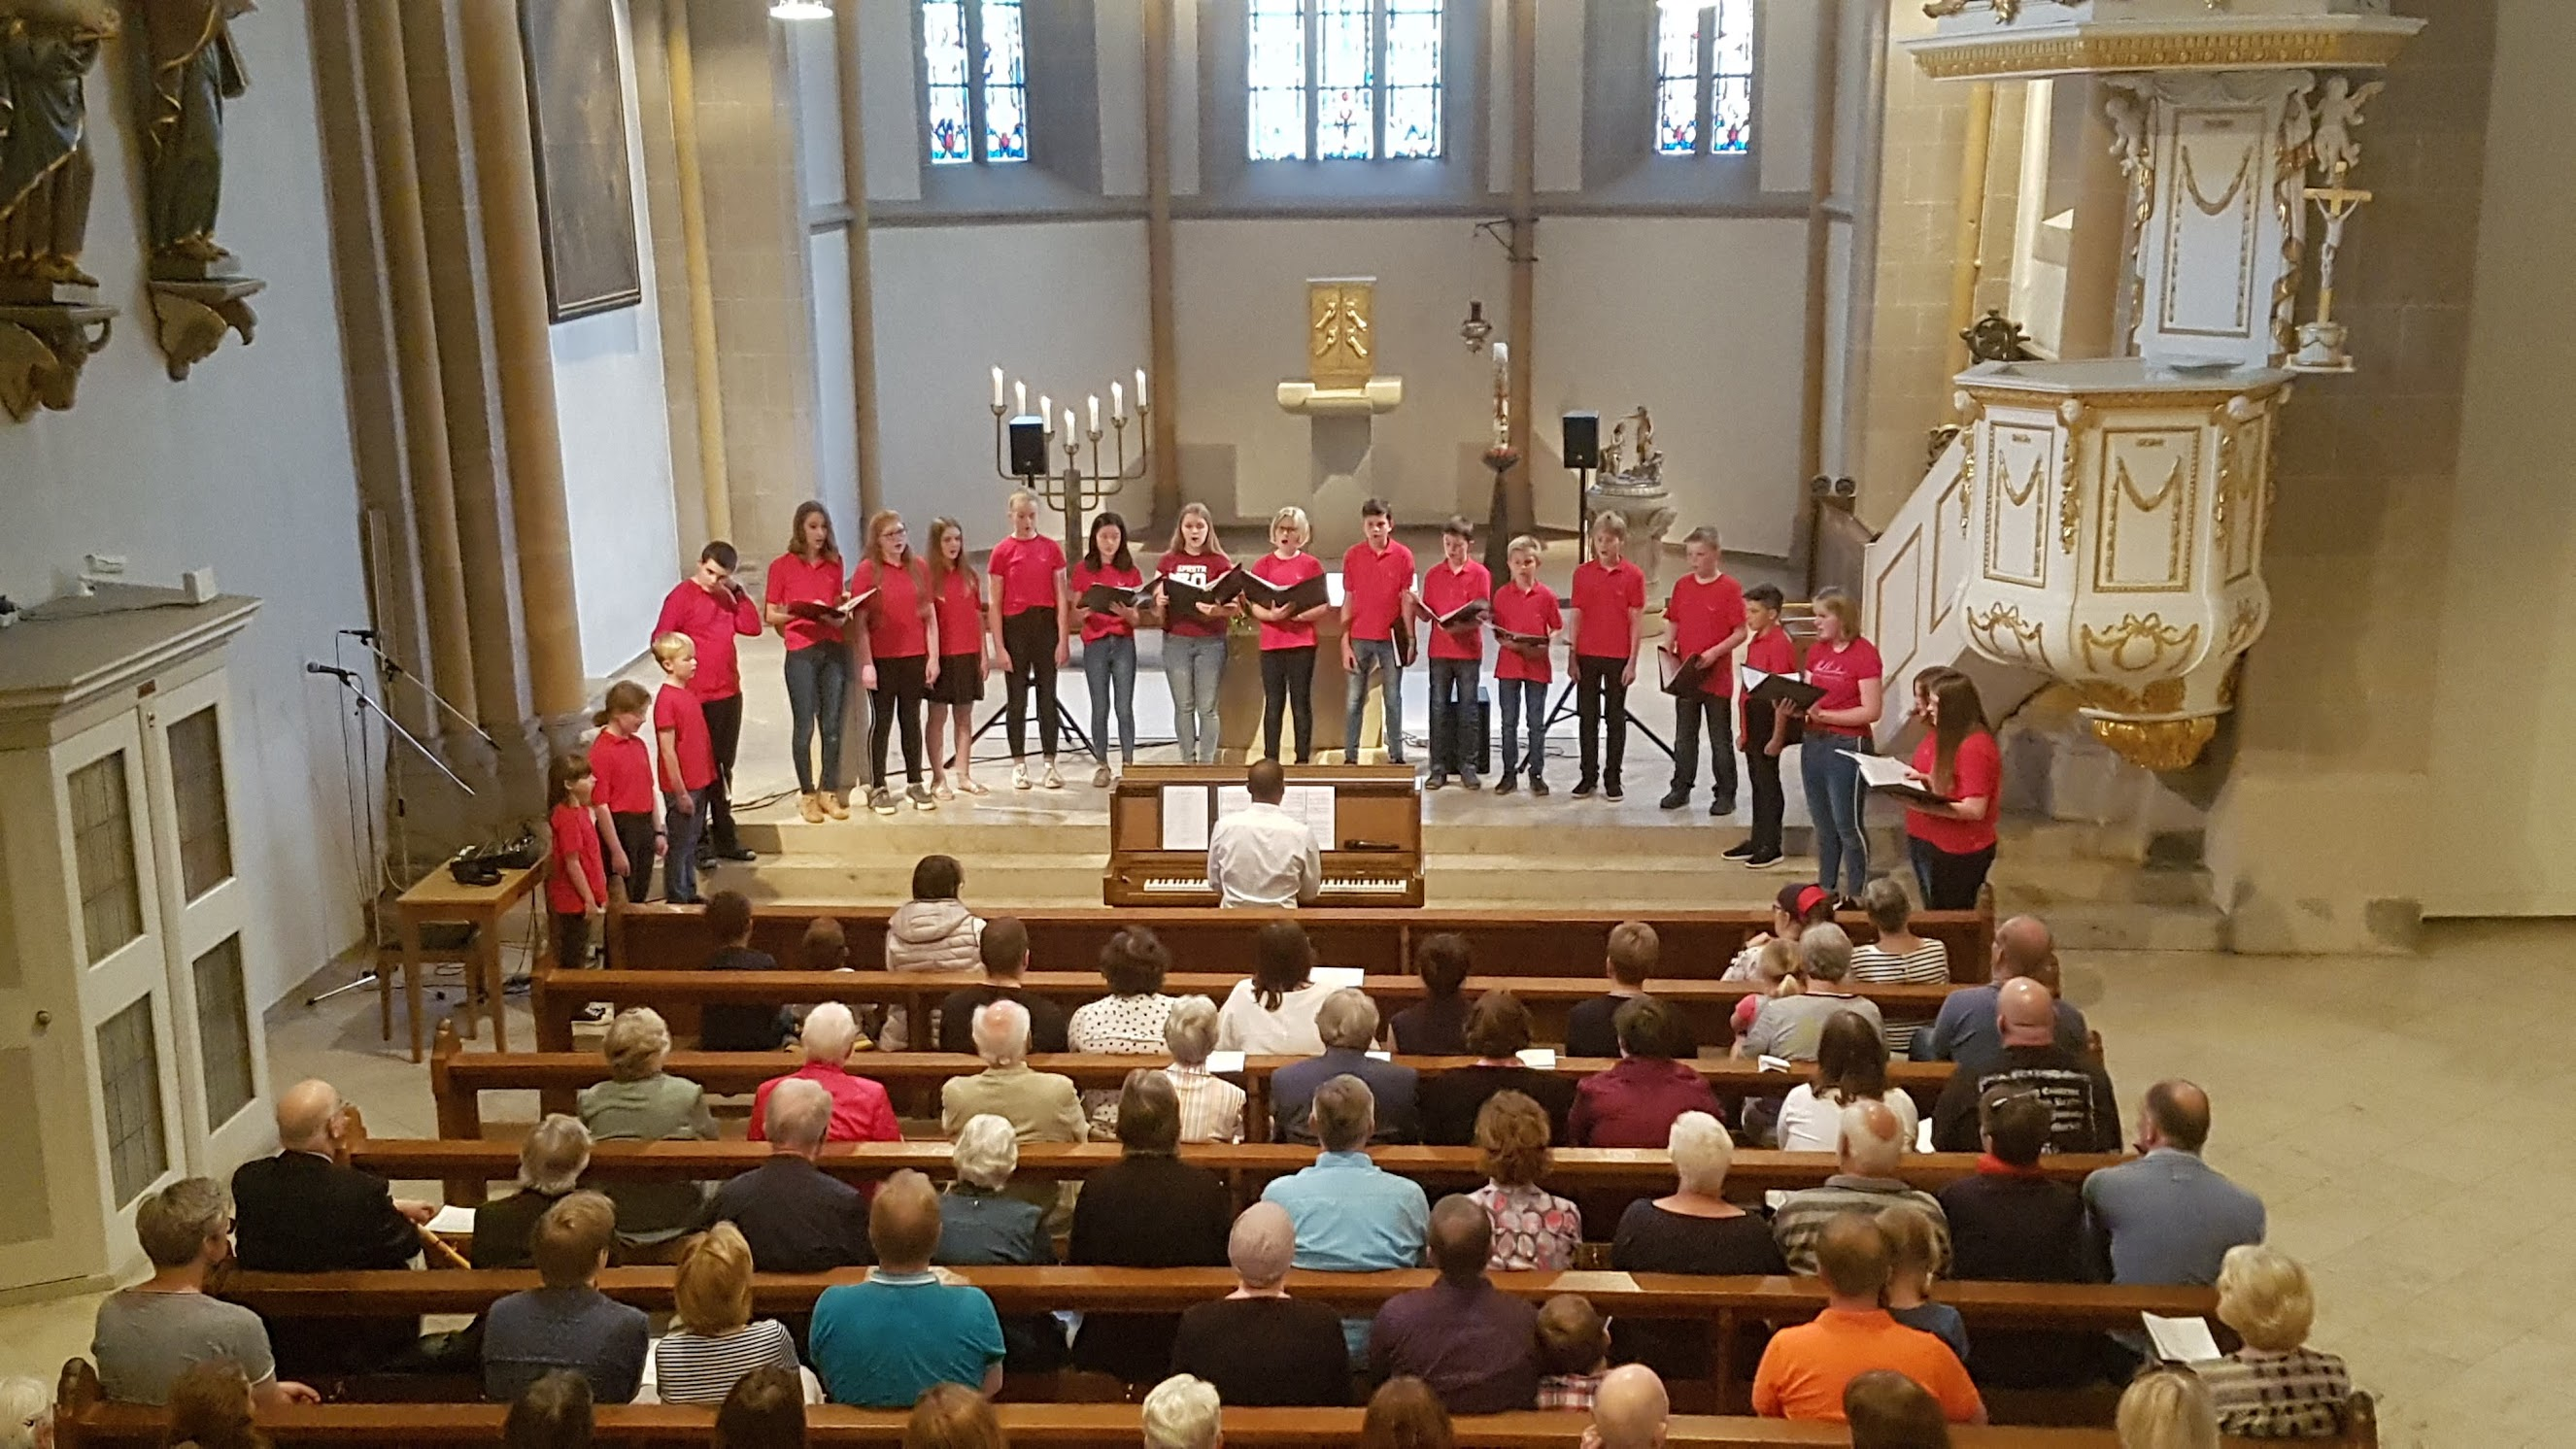
\includegraphics[width=\textwidth]{images/chor.jpg}
\caption{Kinderkantorei St. Matthäus}
\end{figure}

\section{Vorwort}
Vor allem in den letzten Jahren musste ich mich gefühlt überall vorstellen. Im
Bewerbungsprozess, im neuem Arbeitsplatz, allgemein vor neuen Gesichter. Immer
stellte ich mich mit den gleichen Themen vor.

Was ich, wenn überhaupt, nur beiläufig erwähnte, war die Musik. Im Angesicht
dessen, dass Technik und vielleicht Saufen interressantere Themen waren, kam ich
nie wirklich dazu.

Da ich mich ehrlich gesagt nicht wohlfühle, all meine Geheimnis in dieses
Dokument niederzuschreiben, werde ich mich zunächst auf diese eine Sache
beschränken.

\section{Chor}
Gebürtig kam ich aus einer Kleinstadt in Niedersachsen. Bis ich eingeschult 
wurde, war ich musikalisch gesehen nur in der Lage, \glqq Alle meine Entchen
\grqq\ auf ein Klavier oder Keyboard zu spielen.

In der Grundschule kam eines Tages ein Musiker. Für eine lange Zeit glaubte ich, 
dass er musikalisch an der Fernsehserie \glqq Little Amadeus\grqq\ beteiligt
war. Eine Internetrecherche dazu führte aber leider zu keinen Ergebnissen.

Jedenfalls war er ein talentierter Pianist und vom Beruf her Kirchenmusiker.
Damals brachte er uns ein paar Lieder bei, die wir dann in seinem Chor später
weitersungen.

In seinem Chor blieb ich, bis ich für unseren Studiengang \glqq
Embedded Systems\grqq\ wegziehen musste. Das waren also ca. 12 Jahre voller
UNICEF-Konzerte, Kirchenmusik und einigen Ausflügen.

\section{Ich in 10 Jahren}

\begin{table}[h]
\centering
    \begin{tabular}{|| l | r ||}
        \hline
        Vorteile & Nachteile \\
        \hline
        Eigene Fangemeinde & Kein Privatleben \\
        Influencerleben (viele Geschenke) & 
        Eine Herausforderung, da hinzukommen \\
        \hline
    \end{tabular}
\caption{Pros und Cons einer Musikkarriere}
\end{table}

Auch wenn mir das Singen Spaß machte, war es schwer, das mit meinem Alltag
zu vereinbaren.

Weil regelmäßig die Chortermine mit der Arbeit damals kollidierten, legte ich
eine Pause ein, bis ich ein paar Monate später zurückkehrte. Wegen des dualem
Studiums 700 km entfernt von der Heimat und wegen Corona musste ich eine
weitere Zwangspause machen.

In der absehbaren Zukunft werde ich den Bachelor hier an der DHBW absolvieren
und mindestens ein paar Jahre lang in der Firma bleiben. Ich hoffe, dass ich
die Chance bekomme, an aufregenden Projekten zu arbeiten.

\section{DevOps}
Zur Zeit steige ich gerade bei unserem Global Formula Racing Team in das 
Themengebiet rund um DevOps ein. Dafür plane ich, zunächst verschiedene Bücher
zu diesem Thema durchzulesen. Z. B. lese ich zur Zeit eine Übersicht über
DevOps als Ganzes \autocite{devops}. Danach habe ich vor, Bücher zu
verschiedenen Tools zu lesen, also für Docker \autocite{docker}, Ansible 
\autocite{ansible} und GitHub Actions \autocite{github-actions}.

\printbibliography

\end{document}
